\documentclass[9pt,a4paper]{article}

\XeTeXlinebreaklocale "zh"
\XeTeXlinebreakskip = 0pt plus 1pt minus 0.1pt
\usepackage[top=1in,bottom=1in,left=1in,right=1in]{geometry}
\usepackage{float}
\usepackage{fontspec}
\newfontfamily\zhfont[BoldFont=Adobe Heiti Std]{Adobe Song Std}
\newfontfamily\zhpunctfont{Adobe Song Std}
\setmainfont{Times New Roman}
\usepackage{indentfirst}
\usepackage{zhspacing}
\zhspacing

\usepackage{listings}
\lstset{
	frame=shadowbox,
	basicstyle=\footnotesize,
	numbers=left,
	numberstyle=\footnotesize,
	tabsize=2,
	breaklines=true,
	xleftmargin=2em,
	xrightmargin=2em,
	aboveskip=1em,
	showspaces=false
	}
	
\usepackage{framed}   
%%%% 段落首行缩进两个字 %%%%
\makeatletter
\let\@afterindentfalse\@afterindenttrue
\@afterindenttrue
\makeatother
\setlength{\parindent}{2em}  %中文缩进两个汉字位


%%%% 下面的命令重定义页面边距,使其符合中文刊物习惯 %%%%
\addtolength{\topmargin}{-54pt}
\setlength{\oddsidemargin}{0.63cm}  % 3.17cm - 1 inch
\setlength{\evensidemargin}{\oddsidemargin}
\setlength{\textwidth}{14.66cm}
\setlength{\textheight}{24.00cm}    % 24.62

%%%% 下面的命令设置行间距与段落间距 %%%%
\linespread{1.4}
% \setlength{\parskip}{1ex}
\setlength{\parskip}{0.5\baselineskip}


\begin{document}
	
%%%% 重定义 %%%%
\renewcommand{\contentsname}{目录}  % 将Contents改为目录
\renewcommand{\abstractname}{摘要}  % 将Abstract改为摘要
\renewcommand{\refname}{参考文献}   % 将References改为参考文献
\renewcommand{\indexname}{索引}
\renewcommand{\figurename}{图}
\renewcommand{\tablename}{表}
\renewcommand{\appendixname}{附录}
%\renewcommand{\algorithm}{算法}
	
	
%%%% 定义标题格式,包括title,author,affiliation,email等 %%%%
\title{RGB-D SLAM入门 \\ RGB-D SLAM Tutorial \\
	第一讲~~预备知识与cmake}
\author{高~翔\footnote{Email: gaoxiang12@mails.tsinghua.edu.cn}\\[2ex]
	 清华大学自动化系\\[2ex]
}
\maketitle

\section{文档说明}
SLAM,即Simultaneous Localization and Mapping,中文译作同时定位与地图创建,是近几十年里机器人领域有重大发展的研究方向。作为自主机器人的核心技术,SLAM在机器人导航、控制、生产等方面都有着重要的研究意义。尤其在二十一世纪,以视觉传感器为中心的视觉SLAM技术,在理论和方法上都经历了明显的转变与突破,正逐步从实验室研究迈向成熟的市场应用。在国外研究如火如荼之际,它在国内的研究尚处于起步阶段。有关SLAM的中文资料、书籍更是难以一见。然而,随着机器人技术得到国家的重视,越来越多的青年研究者、学生正逐渐跨入这片领域。本文档则试图为这些刚走进SLAM的同事们,提供一些简单而实际的参考。

小萝卜:师兄!你上面写的都是些什么东西啊!

师兄:都是些没什么卵用的废话啊……但是没这些东西文档就不上档次啊。

小萝卜:师兄!你别干这些无聊的事情了!赶紧教我做SLAM啊!

师兄:前言才写了一段,读者会觉得我在敷衍他们的吧。算了,不管了,前两天让你跑的rgbd-slam怎么样了?

小萝卜:跑起来了!然后呢?

师兄:然后你就可以调调参数,改改代码啥的啊。

小萝卜:师兄!我看不懂!

师兄:呃这个……

小萝卜:师兄!你给我写一个SLAM程序吧!

师兄:呃这个……

小萝卜:赶紧写啦师兄!写完了你请我吃饭!

师兄:吃饭啊,那好吧……

于是,师兄就开始写这本文档了。由于师兄也不知道什么时候会写完,所以他每写一段就拿给小萝卜看(然后请他吃饭)。还好小萝卜热情很高,每次师兄给他写好的代码,都拿回去仔细看而且跑了。这也给了师兄很大动力继续往下写。

\section{预备知识}
为什么要写一个SLAM程序,而不采用现有的代码?

-答案是:为了更深的理解。

\begin{enumerate}
	\item 一个完整的程序含有大量的算法与GUI的代码,你读一遍需要多久?弄清楚原理要多久?
	\item 别人工具都做好了,代码都写完了,参数也调好了,你拿过来运行。效果是看出来了,然而接下来怎么办?
	\item 你迟早要自己写代码。
\end{enumerate}

另一方面,自己写程序,不代表要用C++实现矩阵的线性代数。基本的库我们还是会用的。

我们要用的库:
\begin{itemize}
	\item OpenCV.
	\item PCL.
	\item g2o等其他的库,用到了再讲怎么装。
\end{itemize}

编程环境是ubuntu 12.04。建议读者和我们使用一样或类似的环境。如果你\textbf{就是}要用Arch/Fedora/Mac……请你自己配环境。

\subsection{安装OpenCV}
推荐从源代码安装的模式。编译过程需要一点时间。

步骤:
\begin{itemize}
	\item 下载OpenCV源代码: http://opencv.org/downloads.html。目前(2015.6)较好的版本是2.4系列,因为3.0系列还不完善(主要是没文档)。请把它下载到电脑上随意一个目录下。
	\item 在下载过程中,你可以安装依赖项。基本的依赖项是底下那些,直接拷贝到终端执行。
	\begin{lstlisting}[language=sh]
		sudo apt-get install build-essential libgtk2.0-dev libjpeg-dev libtiff4-dev libjasper-dev libopenexr-dev cmake python-dev python-numpy python-tk libtbb-dev libeigen2-dev yasm libfaac-dev libopencore-amrnb-dev libopencore-amrwb-dev libtheora-dev libvorbis-dev libxvidcore-dev libx264-dev libqt4-dev libqt4-opengl-dev sphinx-common texlive-latex-extra libv4l-dev libdc1394-22-dev libavcodec-dev libavformat-dev libswscale-dev
	\end{lstlisting}
	
	\item 把OpenCV解压到下载目录中,用cmake编译再安装:
	\begin{lstlisting}[language=sh]
		mkdir build
		cd build
		cmake ..
		make
		sudo make install
	\end{lstlisting}
	
	编译过程需要一点时间,长短视你机器的配置而定。慢一点的可能一下午就过去了,请顺便找点其他事干干例如看场电影之类的。
	
	小萝卜:装完之后OpenCV在哪里呢?
	
	师兄:头文件在/usr/local/include/,里面有opencv和opencv2的头文件。我们基本只用opencv2啦。
	
	小萝卜:有2谁还用1啊。
	
	师兄:库文件就在/usr/local/lib/下面,当然这些在install的时候都是可以改动的,我列的是默认位置。
	
	小萝卜:师兄!刚才用的cmake是什么东西啊?
	
	师兄:cmake就是linux下的C++管理工具啦。简单的代码你可以用g++一条条敲,再多些可以用Makefile来管理,cmake就是自动生成makefile的工具,比makefile集成度更高一些。
	
	小萝卜:哦好的!我懂了师兄!请我吃饭哦!
	
	师兄:好!
	
	\item PCL
	
	PCL就是Point Cloud Library啦,处理点云的必备工具。
	
	小萝卜:师兄!为什么要处理点云?
	
	师兄:啊……忘了说了,这篇文档是讲RGB-D SLAM的呀,深度相机采出来的本来就是点云数据啦。
	
	小萝卜:这么重要的事情为什么你不放到开头去讲啊!
	
	师兄:我忘了……
	
	不管如何,PCL官网(http://pointclouds.org)上已经给出了ubuntu的安装方法。因为很多开发工具在ubuntu上装起来最方便,也比较适合小萝卜这种新手,所以我们才选用了ubuntu。
	
	要装PCL,请敲以下代码:
	\begin{lstlisting}[language=sh]
	sudo add-apt-repository ppa:v-launchpad-jochen-sprickerhof-de/pcl
	sudo apt-get update
	sudo apt-get install libpcl-all
	\end{lstlisting}
	
	那么,类似的,你能否找到PCL的头文件以及库文件的安装目录呢?
	\begin{framed}  
	\subsection*{小作业}
	请找到PCL的头文件与库文件的安装目录。
	\end{framed}
	
	
	
\end{itemize}

小萝卜:师兄你写东西废话还是这么多~

师兄:我也没办法啊……

\section{Hello SLAM!}
我们已经安装好了OpenCV和PCL,下面我们开始来写第一个程序吧!

小萝卜:终于可以开始写程序喽!我最爱写程序!我感到程序员之魂在我体内燃烧!

师兄:呃,可是我们第一个程序要做什么呢?

小萝卜:我们马上来写SLAM吧!

师兄:可是那样读者能看懂吗……我们还是从简单的东西开始吧。

小萝卜:好!那就写一个简单的SLAM!

首先我们来构建一个CMake项目,作为今后写代码的模板。开头读者可能会觉得困难,但是万事开头难,后来你就慢慢习惯了。

Linux下的CMake项目通常由几个文件夹组成。例如我们今天讲的slam,你可以在机器上建一个叫slam的文件夹(注意:这个文件夹就是你代码的根目录了!)。然后往里面建几个子文件夹:
\begin{framed}
\begin{description}
	\item{bin} 用来放编译好的可执行二进制文件。
	\item{src} 用来放源代码。
	\item{lib} 用来放编译好的库文件。
	\item{include} 用来放头文件。
\end{description}
\end{framed}
为什么要用这种目录结构呢?其实这是一种编译习惯,当然你可以把所有文件都搁一个目录里,但是这样看起来很乱不是么。通常我们把源代码和编译好的东西分开。如果源代码比较多,还会按模板分开。像opencv和pcl的代码就是由好多个模块组成的。

我们要把目录结构告诉cmake。所以我们在代码根目录下写一个CMakeLists.txt。cmake在生成代码时,会读这个文件,并按照它来编译你的代码。刚才我们对opencv进行编译时,也采用了这个步骤。好,现在在代码根目录下新建一个CMakeLists.txt:

\begin{lstlisting}[language=sh]
touch CMakeLists.txt
\end{lstlisting}

打开此文件,写入:
\begin{lstlisting}[language=sh]
	
	CMAKE_MINIMUM_REQUIRED( VERSION 2.8 ) #设定版本
	PROJECT( slam ) #设定工程名
	SET( CMAKE_CXX_COMPILER "g++") #设定编译器
	
	#设定可执行二进制文件的目录
	SET( EXECUTABLE_OUTPUT_PATH ${PROJECT_SOURCE_DIR}/bin) 
	
	#设定存放编译出来的库文件的目录
	SET( LIBRARY_OUTPUT_PATH ${PROJECT_SOURCE_DIR}/lib) 
	#并且把该目录设为连接目录
	LINK_DIRECTORIES( ${PROJECT_SOURCE_DIR}/lib)
	
	#设定头文件目录
	INCLUDE_DIRECTORIES( ${PROJECT_SOURCE_DIR}/include)
	
	#增加子文件夹,也就是进入源代码文件夹继续构建
	ADD_SUBDIRECTORY( ${PROJECT_SOURCE_DIR}/src)
	
\end{lstlisting}

井号后面的是我的注释,只是为了帮助你理解,你可以不敲。通过这个文件,你应该了解了CMakeLists.txt的一些基本的用法。如果你想找一个系统的介绍,附件里提供了《CMake实践》电子书,我认为是一个不错的参考资料。

小萝卜:等一下师兄!库文件和二进制都是什么啊!

师兄:二进制就是可以直接运行的程序啦,库文件呢,就是为这些二进制提供函数的啦。有main函数的代码可以编译成二进制,其他的则编译成库文件。链接时,把库文件链到二进制上,就可以运行啦。

小萝卜:师兄我还是不懂!

师兄:呃,那我们还是通过实例来做吧。在src/文件夹下新建一个main.cpp文件,输入:

\begin{lstlisting}[language=C++]
#include <iostream>

int main(int argc, char**argv)
{
	std::cout<<"Hello SLAM!"<<std::endl;
	return 0;
}
\end{lstlisting}

这当然是个很简单的,一目了然的程序。所以我也没有加注释。然后,我们要从这个源代码生成一个二进制。在src/目录下新建一个CMakeLists.txt,输入:

\begin{lstlisting}[language=sh]
# 增加一个可执行的二进制
ADD_EXECUTABLE( main main.cpp )
\end{lstlisting}

这样,cmake就会把这个main.cpp编译成一个叫做main的二进制了。赶紧来试试吧。首先转到代码根目录下,输入:

\begin{lstlisting}[language=sh]
mkdir bulid
cd build
cmake ..
make
\end{lstlisting}

编译通过的话,就会在bin/目录下生成一个main的二进制哦!

\begin{figure}[!htp]
\centering
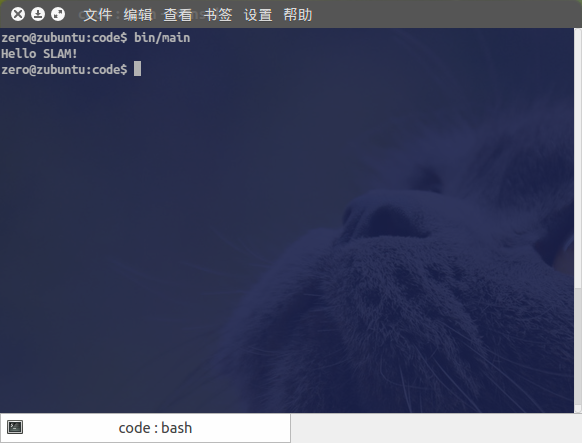
\includegraphics[width=.5\textwidth]{figure/p1.pdf}
\caption{运行main}
\end{figure}

是不是觉得这个程序太简单了?没关系,难的在后面呢!

小萝卜:难道这一讲就这样结束了?

师兄:是啊……毕竟写得还是蛮辛苦的,我得去休息一会。

小萝卜:可是我们基本上没写什么程序啊!

师兄:别急啊,你先把cmake好好学学,之后的工作都得在这上面做。

小萝卜:好吧!那师兄我们下一讲要做什么呢?

师兄:嗯,我们会用opencv读个图,再把它转成点云,怎么样?

小萝卜:听起来不难啊,那下一讲再见啦!

\begin{framed}
未完待续	
\end{framed}
	

\end{document}